\chapter{Drupal} \label{Drupal}
\section{Wat is Drupal?}
\begin{wrapfigure}{r}{0.3\textwidth}
\vspace{-40pt}
%\hspace{-10pt}
\centering
\label{fig:drupalLogo}

\includegraphics[width=0.3\textwidth]{fig/drupalLogo}
\vspace{-30pt}
%\hspace{-10pt}
\centering
\caption{Drupal logo}
\centering
\vspace{-40pt}
\end{wrapfigure}
We kunnen Drupal het best beschrijven aan de hand van Figuur~\ref{fig:watIsDrupal}.
Drupal is een \textit{Content Management System} (CMS)\nomenclature{CMS}{Content Management System}, een \textit{framework} voor webapplicaties en een \textit{social publishing platform}. Maar Drupal is meer dan software alleen. Drupal staat voor een gemeenschap van ontwikkelaars en gebruikers met uiteenlopende doeleinden die elk hun eigen visie willen realiseren.~\cite{drupalDefGuide}

\subsubsection{Content Management System}
Drupal levert alle functies en mogelijkheden van een krachtig CMS. We denken meteen aan het kunnen inloggen en registreren van gebruikers, verschillende soorten gebruikers kunnen defini\"{e}ren, verschillende niveaus van permissies,... Ook denken we aan het cre\"{e}ren, aanpassen, beheren, weergeven, categoriseren en aggregeren van content. Drupal biedt bovendien de mogelijkheid om modulair extra functionaliteit toe te voegen naar eigen noden en wensen.

\subsubsection{Framework voor webapplicaties}
Drupal is zeer flexibel en krachtig waardoor er enorm veel verschillende soorten webapplicaties mee kunnen gebouwd worden. Dit is deels te danken aan de API's die Drupal aanbiedt. Deze worden bij elke versie van Drupal uitgebreid maar ze worden niet complexer om te gebruiken. % Drupal's veelzijdigheid wordt nogmaals bewezen met het feit dat het zowel als \textit{frontend} voor Java-gebaseerde applicaties kan optreden als voor \textit{backend} voor AJAX of Flash-driven \textit{frontend}s.

\subsubsection{Social publishing platform}
Dat Drupal een \textit{social publishing platform} is, houdt in dat content gemakkelijk te delen is via Drupal. Drupal biedt de mogelijkheid complexe data in een structuur te gieten die gemakkelijk uit te wisselen is. Op deze manier is het eenvoudig hetzelfde stuk content voor te stellen op verschillende websites.

\begin{figure}[h]
\centering
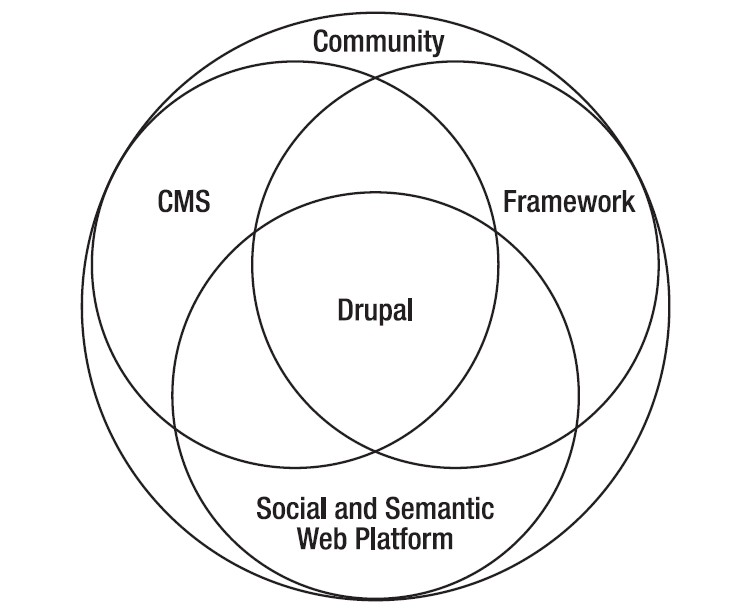
\includegraphics[width=0.4\textwidth]{fig/watIsDrupal}
\caption{Wat is Drupal?}
\vspace{-10pt}
\label{fig:watIsDrupal}
\end{figure}

We kunnen Drupal ook beschrijven als een gratis softwarepakket dat je de mogelijkheid biedt om jouw inhoud gebruiksvriendelijk te beheren en te publiceren. En dit op zo een manier dat je een eindeloze graad van personalisering hebt. Deze inhoud kan bestaan uit allerlei dingen, zoals: een blog, een video, een foto, een artikel, resultaten van een experiment,... Algemeen is dit dus een combinatie van tekst, beelden en audio die bezoekers van je website kunnen zien, lezen en/of horen. Bovendien is Drupal \textit{open source}.\\

Bij de implementatie van Drupal worden een aantal technologie\"{e}n gebruikt. De eerste is de \textit{HTML-embedded} \textit{scripting}taal PHP wat voor PHP: Hypertext Preprocessor staat. Het wordt gebruikt om dynamische webpagina's te cre\"{e}ren. PHP wordt \textit{server-side} uigevoerd, de code wordt op een webserver uitgevoerd. Dit in tegenstelling tot \textit{client-side}talen waar de code in een browser uitgevoerd wordt aan de clientzijde. De syntax van PHP bevat elementen van C, Java en Perl. Vanaf de huidige versie (PHP5) wordt object-ge\"{o}rienteerd programmeren ondersteund. Het is echter nog steeds mogelijk volledig proceduraal te werken.\\

Voor de \textit{frontend} wordt er een noemenswaardige hoeveelheid JavaScript in de vorm van jQuery gebruikt.\\

Als laatste wordt voor het opslaan van content en configuratiegegevens van Drupal een relationele databank gebruikt. Welke specifieke technologie als achterliggende databank gebruikt wordt kan zelf gekozen worden. Door in code gebruik te maken van de Database Abstraction Layer heeft deze keuze geen invloed op de Drupal code. Standaard wordt het gebruik van deze laag in combinatie met MySQL, SQLite of PostgreSQL ondersteund. Indien een andere technologie gekozen wordt, is er extra configuratie nodig. De Database Abstraction Layer wordt verder besproken in \ref{databaseAbstractionLayer}.\\

\noindent
Drupal in zijn huidige versie (7) kan op elk platform draaien onder volgende twee voorwaarden:
\begin{itemize}
\item Het platform bevat een webserver die PHP, en dus \textit{server-side} \textit{scripting} ondersteunt. Voorbeelden van deze webserver zijn:  Apache, IIS, Lighttpd en nginx.
\item Het platform ondersteunt een van volgende databanktechnologie\"{e}n: MySQL, SQLite of PostgreSQL.
\end{itemize}
Bij deze masterproef wordt er gebruik gemaakt van Apache en MySQL.

\subsection{Basiswebsite}
Wanneer je Drupal installeert beschik je meteen over een basiswebsite. Omdat je meteen al een bruikbare website hebt, is de drempel om Drupal te beginnen gebruiken dus laag. Deze website biedt meteen al een heleboel functionaliteit aan die geleverd wordt door de zogenaamde Drupal\textit{core}. %en een aantal out-of-the-boxfuncties.
\begin{figure}[h]
\begin{center}

\includegraphics[keepaspectratio,width=1\textwidth]{fig/drupalBasiswebsite}
\vspace{-10pt}
\caption{Basiswebsite van Drupal met Bartik-theme}
\vspace{-30pt}
\end{center}
\end{figure}

\section{Waarom Drupal?}
We bekijken de principes waarop Drupal gebouwd is \cite{drupalMission}:
\begin{itemize}
\item Modulair en uitbreidbaar: Drupal kan uitgebreid worden met modules, waarbij je zelf ook modules kan ontwerpen indien er nog geen bestaat die aan jouw noden voldoet.
\item Kwaliteitsvolle codering: kwaliteitsvolle, elegante en goed gedocumenteerde code is een prioriteit.
\item \textit{Standard-based}: Drupal maakt gebruik van ingeburgerde standaarden zoals bijvoorbeeld XHTML en CSS.
\item \textit{Low-resource demanding}: om een goede prestatie te garanderen, maakt Drupal gebruik van low-profile codering (bijvoorbeeld minimaliseren van databasequeries).
\item \textit{Open source}: Drupal is gebouwd op, en kan gebruikt worden in, andere \textit{open source}projecten.
\item Gebruiksvriendelijk: Drupal moet gemakkelijk te gebruiken zijn. Zowel voor gebruikers, ontwikkelaars en administrators van een website.
\item Samenwerking: Drupal voorziet systemen om samenwerking te bevorderen, waaronder het versiebeheersysteem GIT.
\end{itemize}

\noindent
Een bijkomend voordeel van Drupal is zijn grote gemeenschap die ondertussen uit al meer dan 630000 actieve gebruikers en ontwerpers bestaat die zich dagelijks inspannen om Drupal steeds beter te maken. Dit aantal neemt elke dag toe. Veel van deze ontwikkelaars werken in hun vrije tijd aan het Drupal concept. Er zijn echter ook een aantal bedrijven die bijdragen leveren. Een van deze bedrijven is Acquia \cite{acquia}, een bedrijf gesticht door Dries Buytaert, de geestelijke vader van Drupal. Acquia biedt een aantal diensten aan voor zowel gebruikers en ontwikkelaars:
\begin{itemize}
\item Er werd gepoogd de drempel om Drupal te gebruiken te verlagen door onder andere de installatie te beperken tot het uitvoeren van een file. \item Begeleiding onder de vorm van video's, extra documentatie, allerlei tutorials en een helpdesk die 24/7 bereikbaar is via mail of telefoon.
\item Elastische resources om \textit{spikes} in netwerkverkeer op te vangen.
\item \textit{Maintenance} van jouw Drupal site.
\end{itemize}

\noindent
We bespreken nu enkele nadelen van Drupal:
\begin{itemize}
\item Aangezien Drupal gebruik maakt van een databank, heb je een databankserver nodig, al dan niet op dezelfde fysieke server als de webserver.
\item Bovendien wordt telkens een pagina wordt opgevraagd, (een stuk van) de \textit{bootstrap}code uitgevoerd, waarbij ook nog eens de databank veelvuldig wordt geraadpleegd. 
Dit maakt Drupal relatief traag.
\item Drupal is zeer gebruiksvriendelijk en ideaal voor de eindgebruikers, die gemakkelijk en interactief inhoud willen toevoegen en beheren. 
Beginnende Drupal ontwikkelaars zullen evenwel merken dat Drupal een erg steile leercurve heeft.
\item Ook ben je afhankelijk van de Drupal gemeenschap en dus de goodwill van de andere leden. Dit is in veel gevallen een voordeel, maar wanneer je een probleem hebt, ben je niet zeker of er wel een oplossing voor bestaat. Indien je gebruik maakt van software verkegen via Acquia heb je dit probleem niet.
\item Tenslotte kan iedereen een module maken. Dit heeft natuurlijk zijn voordelen maar wanneer je een module van iemand anders gebruikt, ben je nooit zeker of de module zal onderhouden worden naar de toekomst toe en of er al dan niet bugs in zitten. Nogmaals, bij gebruik van software verkregen via Acquia is dit minder van toepassing.
\end{itemize}

\section{Werking van Drupal}

Aan de hand van een voorbeeld \cite{drupalDefGuide} proberen we de lezer een idee te geven van de werking van Drupal. Bekijk Drupal als een digitale postzegelsorteerder. Nodes in Drupal zijn te vergelijken met de postzegels en het concept van contenttypes in Drupal is vergelijkbaar met de verschillende soorten postzegels (postzegels van \euro~0,67, \euro~1,34, ... ). Naast contenttypes, kan je \textit{taxonomy} gebruiken om een verdere onderverdeling te maken in de postzegels. De mate waarin en de criteria waarop je je onderverdeling maakt, kan je zelf kiezen (land, kleur, ...). Je kan zelf ook extra criteria opgeven, zoals 'grekegen-van-oma'. Je kan \textit{taxonomy} ook gebruiken om metadata toe te voegen aan content. Views is het mechanisme dat je postzegels sorteert en weergeeft in de vorm van pagina's en \textit{Blocks}. Van deze pagina's en \textit{Blocks} kan je zelf grootte, vorm, kleur en andere criteria opstellen zodat je deze helemaal kan personaliseren. %In paragraaf \ref{drupalBouwstenen} bespreken we de verschillende Drupal concepten in detail.\\

%Het achterliggende design pattern dat gebruikt wordt in Drupal is het Presenstation-Abstraction-Control (PAC) pattern. 

%Zie Figuur~\ref{fig:drupalGrafischeWeergave}.

%\begin{figure}[h]
%\centering
%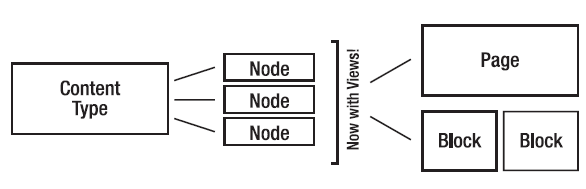
\includegraphics{fig/drupalGrafischeWeergave}
%\centering
%\vspace{-10pt}
%\caption{Grafische weergave van hoe Drupal content aanbiedt}
%\vspace{-10pt}
%\label{fig:drupalGrafischeWeergave}
%\end{figure}

\subsection{Drupal bouwstenen}\label{drupalBouwstenen}
We gaan dieper in op de begrippen die gebruikt werden in het postzegelsorteerdervoorbeeld en lichten enkele extra concepten toe die eveneens belangrijk zijn in Drupal.

\subsubsection{Contenttype}
Een contenttype bepaalt het soort content. Het bundelt soorten gegevens tot een logisch geheel. Wanneer content van een bepaald type wordt aangemaakt, worden de gegevens ingevuld door middel van \textit{Fields}. De toegevoegde content wordt een node genoemd. Ook biedt een contenttype de mogelijkheid om verschillende soorten content te onderscheiden van elkaar op basis van het type.
Drupal biedt gebruikers de mogelijkheid aan om hun eigen \textit{custom} contenttypes te maken. Hoe contenttypes aangemaakt en verwijderd worden wordt in paragraaf \ref{contenttypeManipulatie}.
%figuur van add contenttype

\subsubsection{Fields}
Via \textit{Fields} kan je gegevens van een contenttype invullen. Standaard biedt Drupal een aantal velden aan om gegevens toe te voegen, zoals een tekstveld of een veld om een afbeelding mee te oploaden. Maar soms schieten deze velden tekort, bijvoorbeeld wanneer je een kalender met drie drop-downlists wil combineren om een datum en tijdstip bij elkaar te laten horen in een veld. Daarom heeft een gebruiker de mogelijkheid \textit{custom} velden te maken. Fields worden verder besproken in paragraaf~\ref{Fields}.

\subsubsection{Node}
Nodes zijn instanties van een contenttype. Een node kan maar aan \'{e}\'{e}n contenttype toebehoren.
Alle nodes hebben enkele eigenschappen gemeenschappelijk:
\begin{itemize}
\item Node id: zorgt voor een unieke identificatie.
\item Menu-instellingen: hier kan je een optionele menulink instellen zodanig dat je het menu op je website volledig kan personaliseren.
\item Mogelijkheden in verband met revisie: in de levensloop van de content kan je revisies maken zodat je terug kan keren naar een vorig moment indien er iets fout gaat met de content.
\item \textit{Uniform Resource Locator} (URL) \nomenclature{URL}{Uniform Resource Locator} pad instellingen: standaard is content beschikbaar via een URL van de vorm /node/node\_id. Maar via deze instellingen kan je een alias opgeven waarlangs de content ook (en dus gemakkelijker) beschikbaar is, dit principe heet in Drupal "\textit{Clean} URL's". De URL zal dan van de vorm /alias zijn.
\item Commentaarinstellingen: je kan zelf instellen of gebruikers commentaar kunnen achterlaten bij deze node.
\item Auteurinstellingen: hier stel je in of de creatietijd en auteur getoond moeten worden bij deze node.
\item Publicatieinstellingen: soms is het mogelijk dat je deze content nog niet beschikbaar wil stellen op de website, of je wil ze tijdelijk offline halen. Via deze instellingen is dit mogelijk.
\end{itemize}

\subsubsection{View}
\textit{Views} worden gebruikt om content visueel voor te stellen op welke manier dan ook. Een \textit{view} is dan ook niet meer dan een visuele representatie van een verzameling content uit de databank.

\subsubsection{Block}
\textit{Blocks} zijn, zoals de naam impliceert, blokken die een verzameling van herbruikbare content bevatten. Ze geven het beeld van die content. \textit{Blocks} kunnen op gemakkelijke wijze toegevoegd worden aan je website waar jij dat wilt en hoe vaak je dat wilt. Het is bijvoorbeeld gemakkelijk om aan te geven dat je een bepaald \textit{Block} enkel op een bepaalde pagina wil laten verschijnen, en bovendien waar op de pagina je dat wilt. Merk echter wel op dat het hier niet echt content betreft, de inhoud van het \textit{Block} wordt aangemaakt bij opvraging en is dus geen blok beheerbare content. We zien een voorbeeld van een \textit{Block} in paragraaf~\ref{jQuery}.

\subsubsection{Theme}
\textit{Themes} zijn templates die bepalen hoe jouw website eruit ziet en aanvoelt voor de gebruiker. Net zoals modules zijn \textit{themes} modulair en zijn ze dus gemakkelijk te wisselen, ook \textit{themes} kunnen zelf ontwikkeld worden en zijn ter beschikking op de Drupal gemeenschap.

\subsubsection{Taxonomy}
Taxonomy geeft je de mogelijkheid om eigenschappen en categorie\"{e}n toe te voegen aan je content, zodat bijvoorbeeld een gebruiker content kan filteren uit een grote verzameling. Het biedt dus een manier om je content te organiseren. Een praktijkvoorbeeld is een receptensite, een gebruiker kan dan recepten filteren aan de hand van de eigenschappen van het gerecht (ingredi\"{e}nten, moeilijkheid, ...).

\subsubsection{Module}
Modules bieden de mogelijkheid om extra functionaliteit in te pluggen op een website. Modules zijn gratis te downloaden van de Drupal gemeenschap en omdat deze gemeenschap groot is, is de kans zeer groot dat er al een module gemaakt is voor jouw probleem. Indien dit niet het geval is, heb je nog altijd de mogelijkheid om zelf een module te ontwikkelen. Het gebruik van modules voorkomt ook dat functionaliteit die je niet nodig hebt, ook niet op jouw website komt. Je website is dus zeer configureerbaar naar eigen wensen (Zie figuur~\ref{fig:drupalOrganizeModules}).
\begin{figure}[h]
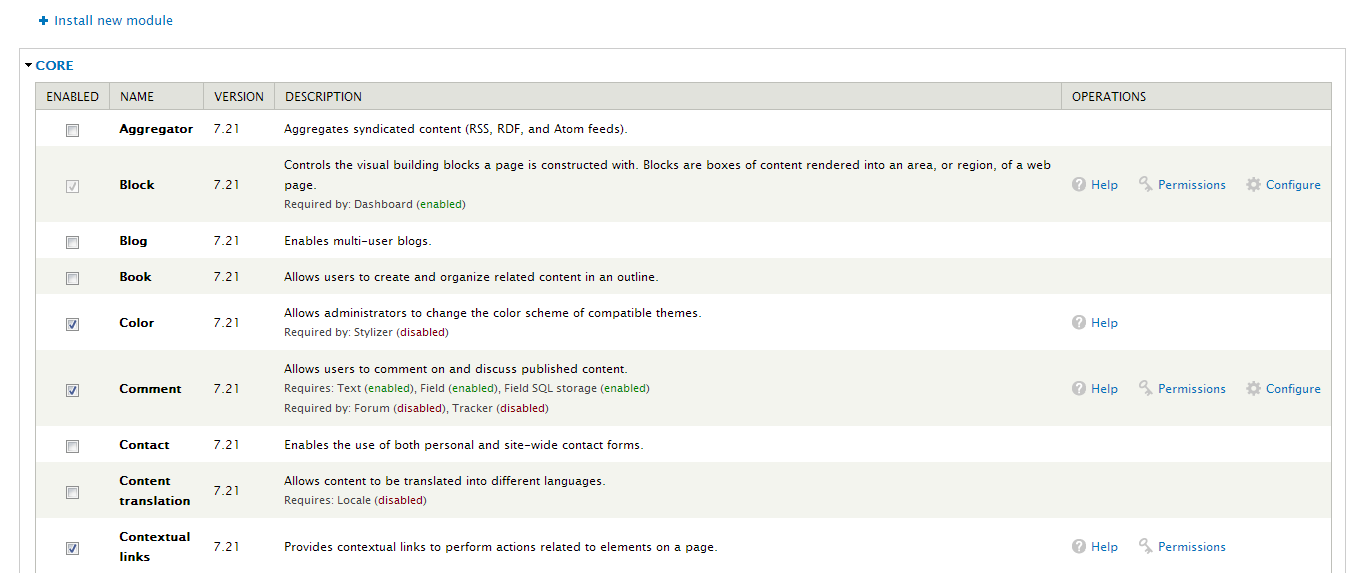
\includegraphics[width=1\textwidth]{fig/drupalOrganizeModules}
\caption{Organisatie van Drupal modules}
\label{fig:drupalOrganizeModules}
\end{figure}

\subsubsection{Gebruikers, rollen en permissies}
%Gebruikers zijn personen die zich aangemeld hebben op jouw website, met uitzondering van de anonieme gebruikers.
Alle gebruikerfunctionaliteit zoals registreren, inloggen, enz... zit reeds in de Drupal \textit{core}. Rollen geven weer tot welk type een gebruiker hoort. Meerdere gebruikers kunnen dezelfde rol hebben, en een gebruiker kan meerdere rollen hebben. Met permissies kan je aangeven welke privileges een gebruiker met een bepaalde rol heeft en dus wat die gebruiker wel en niet mag doen. Deze permissies worden gekoppeld aan een rol zodat alle gebruikers die deze rol hebben automatisch de privileges hebben van deze rol. Drupal biedt standaard drie rollen aan: de Administratorrol, die alle privileges bevat; de geauthenticeerde gebruikerrol, die een aantal van de privileges van de Administratorrol bevat en de anonieme gebruikerrol, die een subset van de privileges van de geauthenticeerde gebruikerrol bevat. Anonieme gebruikers zijn gebruikers die zich niet aangemeld hebben op de website.

\subsubsection{Hooks}
Hooks zijn functies die gedefinieerd zijn door de Drupal \textit{core}. Ze kunnen worden ge\"{i}mplementeerd door elke module. In de Drupal \textit{bootstrap} zal de Drupal \textit{core} dan op bepaalde tijdstippen de bijhorende \textit{hooks} oproepen van elke module die de \textit{hook} ge\"{i}mplementeerd heeft. Hiervoor wordt een zeer eenvoudig mechanisme gehanteerd. Een module kan zo'n \textit{hook} implementeren door de naam van de \textit{hook} te laten voorafgaan door de naam van de module die de \textit{hook} implementeert (zie codevoorbeeld~\ref{lst:drupalHookExample}).\\

\scriptsize
\lstset{language=PHP}
\begin{lstlisting}[label=lst:drupalHookExample,caption=Implementatie van hook\_node\_view door de module coap\_sensor]
function coap_sensor_node_view($node, $view_mode, $langcode) {
  if($node->type == 'coap_resource'){
    _coap_resource_add_js();
  }
  else if($node->type == 'coap_device'){
    $node->content['coap_device_form'] = drupal_get_form('coap_device_form', $node);
  }
  return $node;
}
\end{lstlisting}
\normalsize

\subsubsection{Entities}
Een nieuw belangrijk concept in Drupal 7 is \textit{entities} \cite{entities}. Dit nieuwe concept in combinatie met de \textit{Entity API} heeft twee positieve effecten. Het eerste effect is dat gebruikers en commentaren dezelfde mogelijkheden krijgen als nodes. In vorige versies van Drupal was het niet mogelijk versies te cre\"{e}ren of velden toe te voegen aan gebruikers of commentaren. Andere voordelen zoals het gebruiken van \textit{views} in combinatie met gebruikers of commentaren was ook niet mogelijk. Het andere effect is het invoeren van object-ge\"{o}rienteerd programmeren van \textit{entities}. Vroeger was het nodig specifieke functies van de \textit{core} te gebruiken om content te bewerken. Een voorbeeld hiervan is node\_save() dat nodes opslaat. Deze functie was enkel toepasbaar op een node. Het alternatief bij de \textit{Entity API} is entity\_save(). Deze functie is niet gelimiteerd tot enkel content of enkel tot gebruikers.
Het is ook mogelijk nieuwe \textit{entities} te maken. %, we gaan hier dieper op in in hoofdstuk~\ref{uitbreidingen}.

\subsubsection{Drupal core}
De Drupal \textit{core} is wat je downloadt van de Drupal website. Het vormt de basis en een uitgebreide \textit{out-of-the-box} functionaliteit, het fungeert eigenlijk als de motor achter een Drupal website. De Drupal \textit{core} is zeer uitgebreid en complex, het vormt op zich al voldoende materiaal voor een scriptie, er verder op ingaan zou ons dus te ver leiden.

\newpage
\subsection{Laadcyclus van de pagina}
Wanneer een webbrowser een Drupal pagina opvraagt, wordt de Drupal URL van de pagina gebruikt. Deze heeft vaak volgende vorm: http://drupalvoorbeeld.org/node/15. De webserver vormt deze URL om naar de vorm: index.php?q=node/15 en geeft dan het pad node/15 door aan Drupal's index.php waarvan de code uitgevoerd wordt. Het uitvoeren van deze code resulteert in een reeks complexe stappen die als eindresultaat de gerenderde pagina hebben. Afhankelijk van het feit of de pagina al dan niet in de cache aanwezig is, verlopen deze stappen anders. Indien de pagina niet aanwezig is in de cache, wordt de volledige \textit{bootstrap} en de \textit{page callback} uitgevoerd. De \textit{bootstrap} bestaat steeds uit dezelfde reeks van acht verschillende fasen die we verder nader toelichten. Na de \textit{bootstrap} wordt de \textit{page callback} uitgevoerd die geassocieerd wordt met het pad meegegeven met index.php. Indien de pagina wel in de cache aanwezig is, wordt er enkel een aantal van de stappen van de \textit{bootstrap} uitgevoerd. De \textit{page callback} wordt in dit geval niet uitgevoerd. We bespreken elke stap van het proces apart, het hele proces wordt weergegeven in Figuur~\ref{fig:drupalPageRendering}.

\begin{figure}
\centering
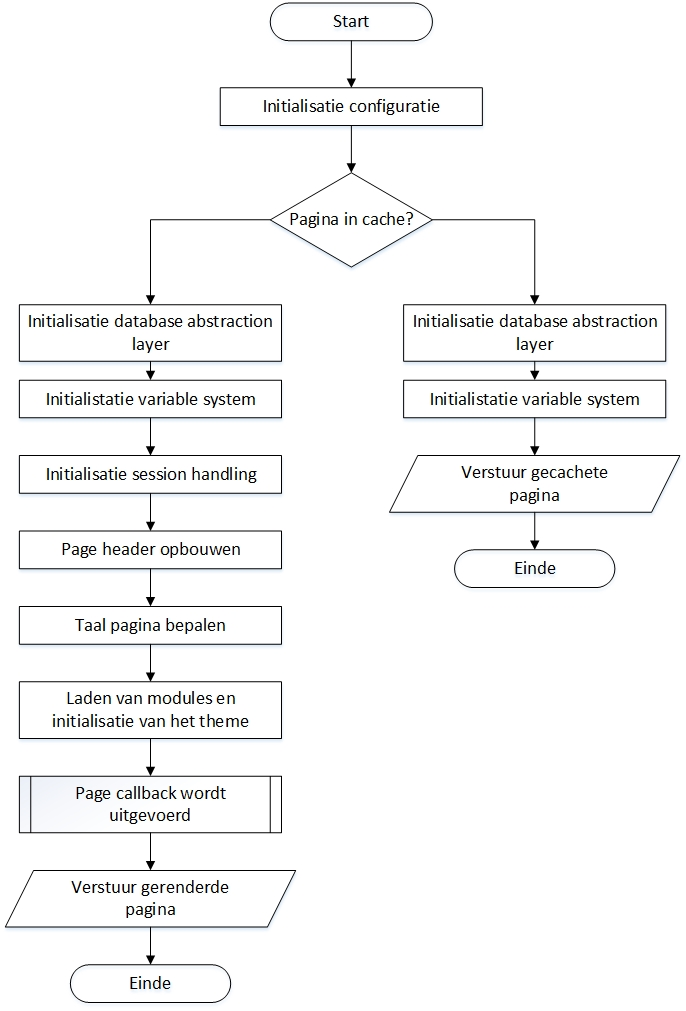
\includegraphics[width=1\textwidth]{fig/drupalPageRendering}
\caption{Laadcyclus van de pagina in Drupal}
\label{fig:drupalPageRendering}
\end{figure}

\subsubsection{Initialisatie van de configuratie}
Deze fase houdt onder andere in dat globale variabelen worden gezet, zoals de basis-URL van de website. Sommige waarden van deze variabelen worden rechtstreeks uit het configuratiebestand settings.php gehaald. Andere worden berekend aan hand van de omgeving waarin de server zich bevindt. In settings.php worden variabelen op opgegeven via de variabele \$conf. Deze variabele is een associatieve array die alle waarden op de variabelenaam mapt.

\subsubsection{Poging tot opvragen van een gecachte pagina}
Caching van pagina's treedt op indien page caching ge\"{e}nabled is. Bovendien gebeurt dit standaard enkel voor anonieme gebruikers. Er zijn echter modules beschikbaar om dit ook voor geauthenticeerde gebruikers te laten gebeuren. Het doel van caching is vermijden dat de volledige \textit{bootstrap} en \textit{page callback} moeten worden doorlopen om zo tijdswinst te cre\"{e}ren. De pagina  wordt enkel uit de cache gehaald als ze eerder is opgevraagd en nog steeds geldig is. De \textit{cache backend} is pluggable en standaard gebruikt Drupal een databank cache implementatie. Deze \textit{cache backend} heeft dus een databankconnectie nodig om de pagina op te halen. Daarom worden de volgende twee fasen (initialisatie van de Database Abstraction Layer en initialisatie van het Variable System) uitgevoerd voor de pagina effectief uit de cache kan gehaald worden. Dit wordt aangegeven door de stippellijnkaders in Figuur~\ref{fig:drupalPageRendering}. De \textit{cache backend} en of caching al da niet ge\"{e}nabled is, wordt opgegeven in settings.php.

\subsubsection{Initialisatie van de Database Abstraction Layer}
Er zijn nog geen verbindingen met de databank nodig. Daarom worden enkel basisklassen en functies ge\"{i}nitialiseerd. Gebruik van de Database Abstraction Layer werd beproken in paragraaf~\ref{databaseAbstractionLayer}.

\subsubsection{Initialisatie van het Variable System}
In deze fase wordt gebruik gemaakt van de \textit{variable}tabel. Deze tabel heeft maar twee kolommen, \textit{name} en \textit{value} en beschrijft, zoals de naam zegt, variabelen. Alle name-valueparen worden uit de \textit{variable}tabel gehaald en toegevoegd aan de variabelen gedefin\"{i}eerd in settings.php. Variabelen die al gedefin\"{i}eerd zijn in settings.php hebben een hogere prioriteit dan degene die uit de \textit{variable}tabel gehaald worden. Het nut van deze variabelen is configuratie toevoegen aan de Drupal website. De reden dat een tabel gebruikt wordt om deze variabelen op te slaan is om de waarden persistent te maken. Wanneer de site offline gaat en terug online komt is de configuratie nog steeds beschikbaar. Drupal biedt ontwikkelaars een aantal functies aan om deze variabelen te manipuleren vanuit code:
\begin{itemize}
\item variable\_get(\$naam, \$default = NULL): De variabele wordt uit \$conf gehaald. Indien deze niet gedefin\"{i}eerd is wordt de waarde in \$default teruggegeven.
\item variable\_set(\$naam, \$value): De variabele wordt opgeslaan in \textit{variable}tabel en gezet in \$conf.
\item variable\_del(\$naam): De variabele wordt verwijderd uit de \textit{variable}tabel en uit \$conf.
\end{itemize}

\noindent
Naast alle variabelen worden de modules die nodig zijn in de \textit{bootstrap} geladen. Onder deze modules verstaan we modules die minstens een van volgende \textit{hooks} implementeerd: hook\_boot(), hook\_exit(), hook\_language\_init(), of hook\_watchdog(). Als laatste onderdeel van deze fase wordt het \textit{locking}mechanisme ge\"{i}nitialiseerd. Dit is nodig bij langdurige processen die parallel naast elkaar kunnen maar niet mogen uitgevoerd worden, we gaan hier niet verder op in.

\subsubsection{Initialisatie Session Handling}
In deze fase wordt aan elke geauthenticeerde gebruiker een sessie gekoppeld. Een anonieme gebruiker krijgt geen sessie toegewezen tenzij er iets in de sessie moet worden opgeslagen. In dat geval wordt een nieuw sessie ID gegenereerd en wordt een nieuw \textit{User}object gecre\"{e}rd met user id 0. Een andere manier dan de standaard databank gebasseerde manier om sessies af te handelen kan opgegeven worden in settings.php.

\subsubsection{Page Header opbouwen}
De eerste HTTP-\textit{headers} worden opgebouwd. Deze worden echter nog niet verstuurd, dit gebeurt pas op het einde van de cyclus. In deze fase vormt zich de eerste mogelijkheid voor modules om functionaliteit in te pluggen in de cyclus van het laden van de pagina. Dit gebeurt via hook\_boot(). Deze \textit{hook} wordt uitgevoerd voor het aanmaken van de HTTP-\textit{headers}.

\subsubsection{De taal van de pagina bepalen}
Als de website meerdere talen ondersteunt wordt in deze fase de gekozen taal van de gebruiker bepaald. Eens de gekozen taal vastgesteld is kunnen implemenaties van hook\_language\_init() gebruikt worden om taalafhankelijke variabelen in te stellen.

\subsubsection{Laden van modules en initialisatie van het theme}
Alle ge\"{e}nablede modules worden geladen en het \textit{theme} wordt ge\"{i}nitialiseerd. Modules hebben nog de kans nieuwe \textit{stream wrappers} toe te voegen en bestaande te wijzigen via de \textit{hooks} hook\_stream\_wrappers() en hook\_stream\_wrappers\_alter(). Met de hook hook\_url\_inbound\_alter() kunnen er wijzigingen uitgevoerd worden aan de URL die gebruikt werd om deze pagina op te roepen. Bij het instellen van het thema wordt gekeken wat het actieve thema is. Dit kan het default thema zijn, ingesteld met de UI, een thema gekozen door de gebruiker ingesteld met hook\_custom\_theme() of een thema specifiek gezet voor dit pad. Aan het einde van deze fase wordt hook\_init() opgeroepen. Dit wordt meestal gebruikt om globale parameters in te stellen die later in de request gebruikt worden.

\subsubsection{Uitvoeren van page callback}
Na het uitvoeren van de \textit{bootstrap} moet de pagina opgebouwd en gerenderd worden. Deze fase leggen we uit aan de hand van een voorbeeld.

\subsubsection{Voorbeeld}
We gaan uit van de specifieke URL http://drupalvoorbeeld.org/node/15 die we in het begin van deze paragraaf gebruikten. Op Figuur~\ref{fig:drupalPageCallback} zijn de hooks waarmee modules tussen beide kunnen komen worden aangegeven naast de respectievelijke fasen.\\

Drupal herkent het woord node in het pad en laadt de node met Node id = 15 via de functie node\_load(15). Gegevens van het node-object worden uit de databank gehaald en de hooks hook\_load(), hook\_entity\_load() en hook\_node\_load() worden opgeroepen zodat modules de kans krijgen het node-object te veranderen of extra acties te ondernemen. Tijdens het laden van de node worden velden geassocieerd met de node eveneens opgehaald. Dit gebeurt met field\_attach\_load(). Modules krijgen de kans de opgehaalde data van de velden te manipuleren met de hooks hook\_field\_storage\_pre\_load() en hook\_field\_attach\_load().\\

Nadat de node geladen is wordt hij doorgegeven aan de \textit{page callback}. Hier wordt hij omgevormd tot een \textit{renderable array}. Dit gebeurt met de functie node\_page\_view(). Het zet als paginatitel de titel van de node. Het voegt ook een canonical en short link toe aan de HTML head elemeents en de HTTP headers. In deze functie wordt de functie node\_show() gebruikt waarin de functie node\_view\_multiple() opgeroepen wordt die op zijn beurt node\_view() oproept waarin uiteindelijk de \textit{renderable array} gemaakt wordt. Via de hooks hook\_node\_view() en hook\_entity\_view() kunnen modules de \textit{renderable array} nog manipuleren. Met de hooks hook\_node\_view\_alter() en hook\_entity\_view\_alter() krijgen modules nog een kans om de array te manipuleren nadat andere modules al veranderingen doorgevoerd hebben.\\

Wanneer de \textit{renderable array} gemaakt is, en teruggegeven wordt door de \textit{page callback}, wordt hij doorgestuurd naar drupal\_deliver\_page() waarin drupal\_deliver\_html\_page() opgeroepen wordt die op zijn beurt de array rendert met drupal\_render(). Voor drupal\_render() effectief opgeroepen wordt, kunnen modules nog wijzigingen doorvoeren met de hook hook\_page\_build(). Modules kunnen nog een laatste keer tussenbeide komen met de hook hook\_page\_alter().

\begin{figure}
\centering
\hspace{55pt}
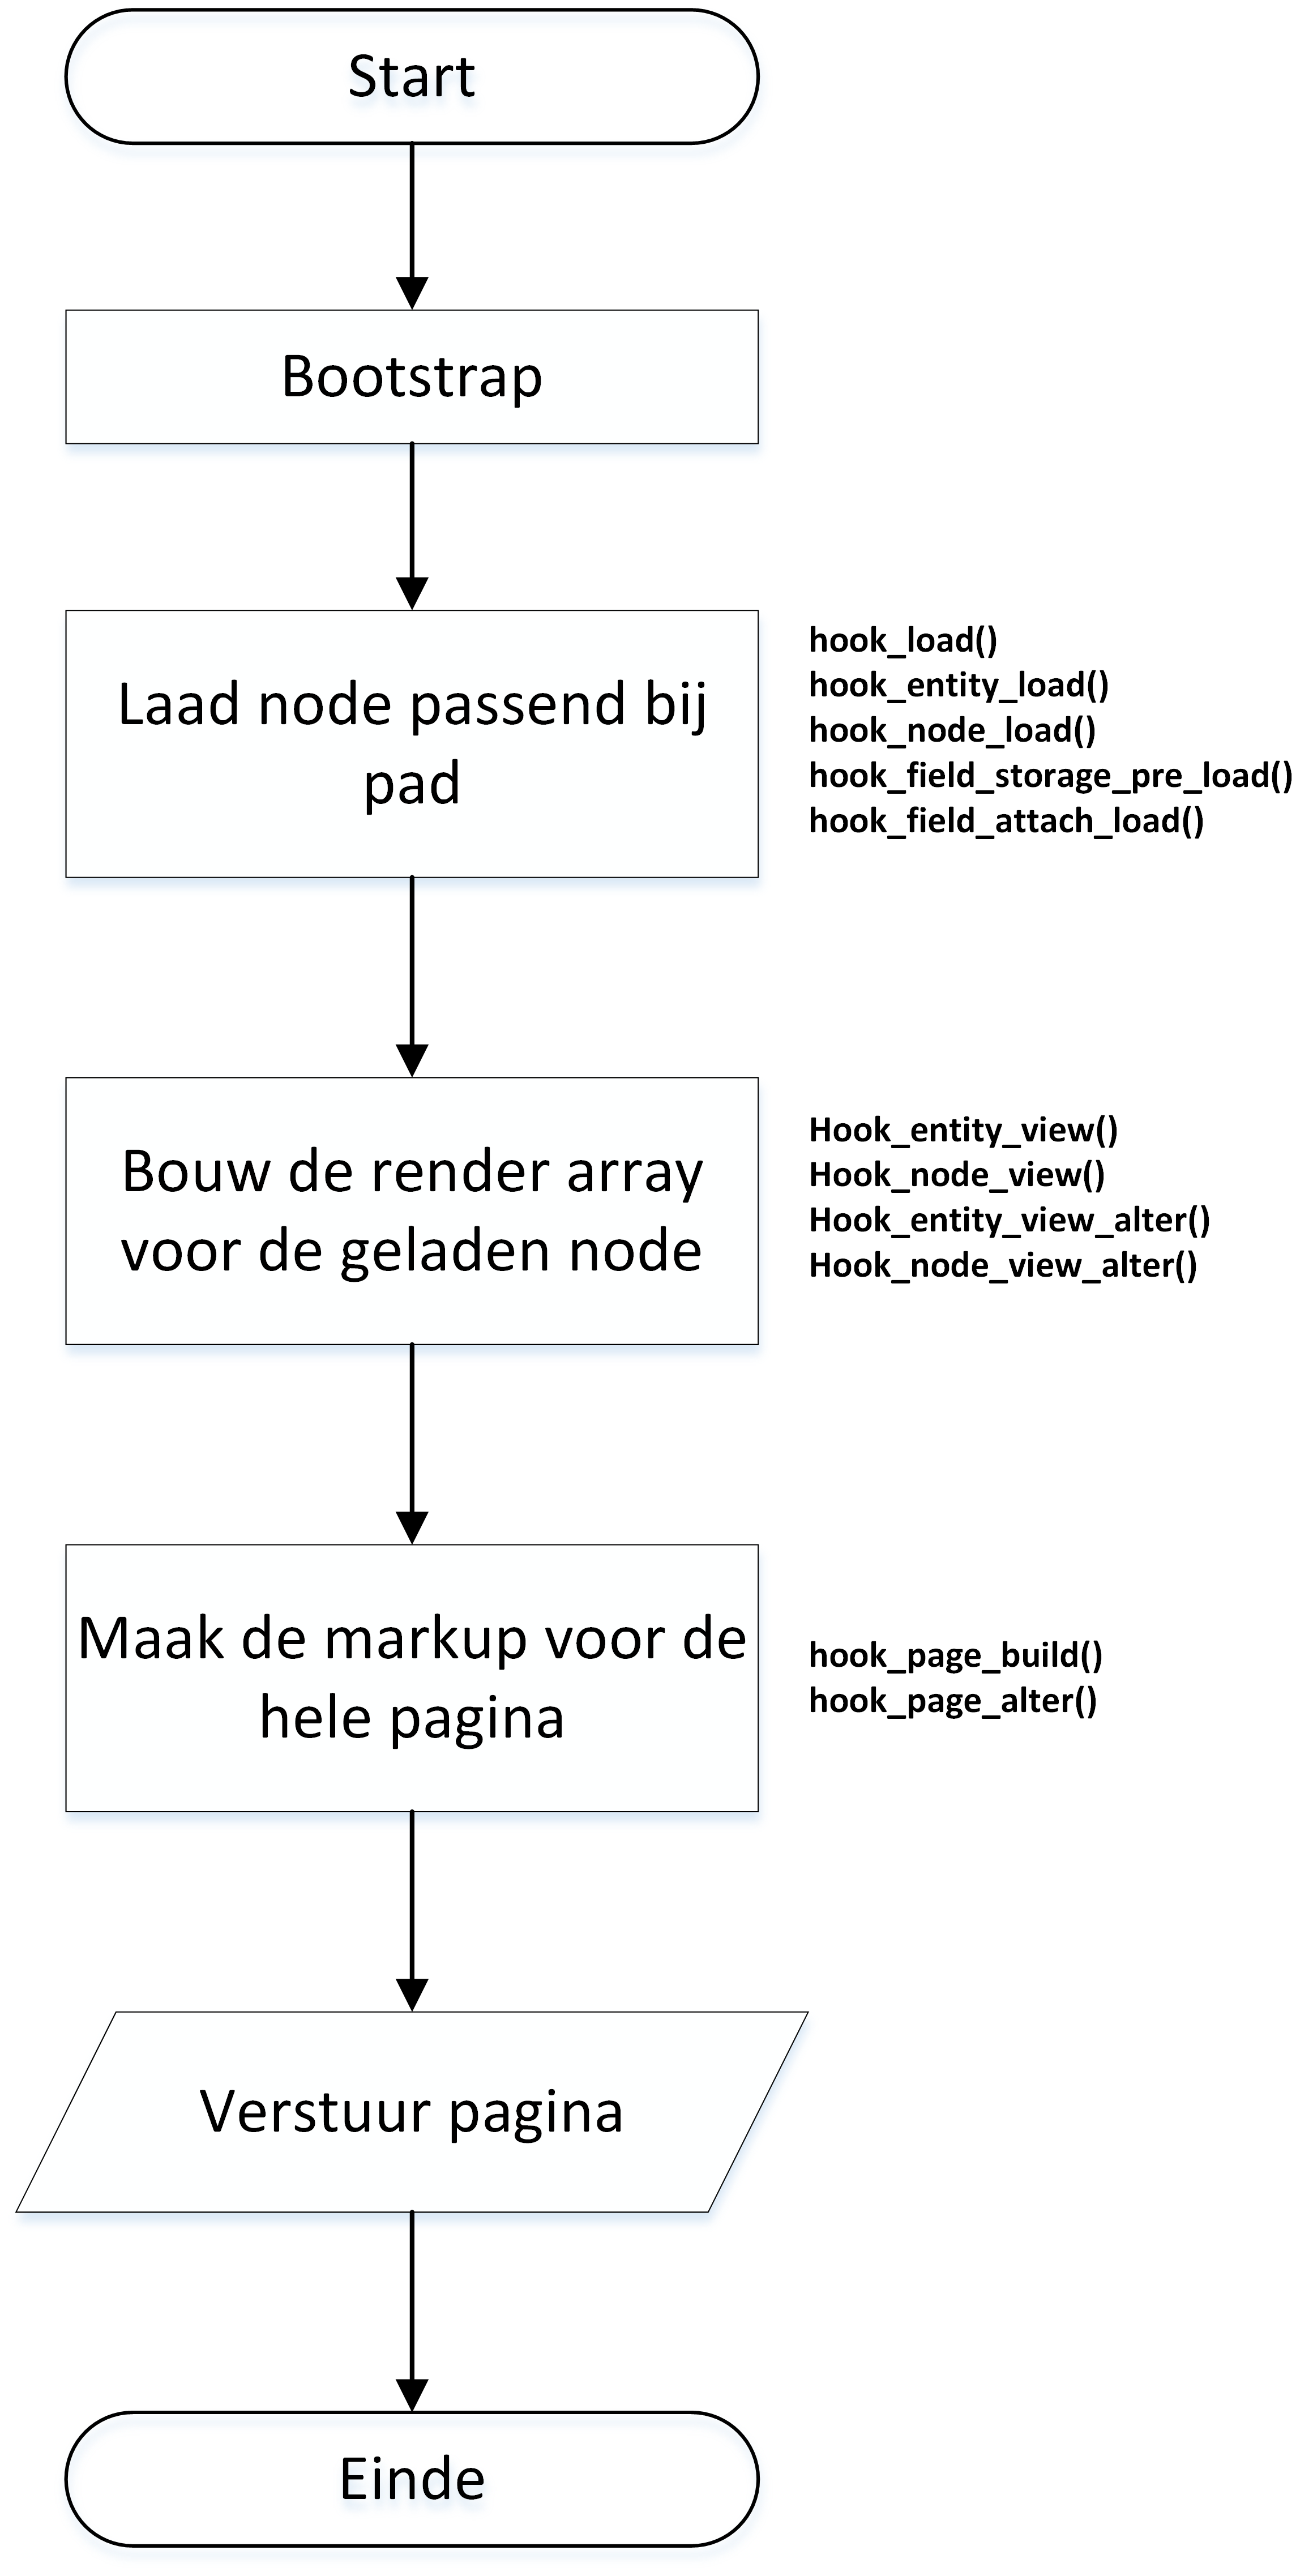
\includegraphics[width=0.65\textwidth]{fig/pageCallback}
\hspace{-50pt}
\caption{Voorbeeld van de laadcyclus van een pagina waar een node weergegeven wordt}
\label{fig:drupalPageCallback}
\end{figure}

\newpage

\subsection{Fields}\label{Fields}
Velden worden op een bepaalde manier behandeld in Drupal. We kunnen velden vergelijken met klassen. Wanneer een veld gebruikt wordt in een contenttype, wordt een instantie van deze klasse gemaakt. De gegevens van velden en hun instanties worden in verschillende tabellen in de databank opgeslaan.
\subsubsection{Fields in de databank}
De verschillende tabellen worden weergegeven in Figuur~\ref{fig:fieldtabellen}. We geven een korte beschrijving van deze tabellen:
\begin{itemize}
\item field\_config: Bevat algemene informatie over een veld. Een veld staat hier maar een keer in beschreven omdat deze informatie onafhankelijk is van de module waarin het gebruikt wordt.
\item field\_config\_instance: Bevat rijen per instantie van een veld. Een veld komt hier evenveel in voor als het aantal modules waarin het gebruikt wordt, rekening houdend met het aantal keer het voorkomt in een module. De informatie beschrijft dus de relatie tussen het veld en de modules waarin het voorkomt.
\item field\_data\_\textit{naam\_field}: Bevat de data bijhorende bij het veld. Data afkomstig van instanties die tot verschillende modules behoren worden in deze tabel opgeslaan. Er worden dus geen aparte datatabellen voorzien per instantie.
\item field\_revision\_\textit{naam\_field}: Bevat archiveringswaarden bijhorende bij verschillende \textit{revisions} van een instantie van een veld zodat teruggekeerd kan worden naar een vorige \textit{revision}.
\end{itemize}
\begin{figure}[h]
\centering
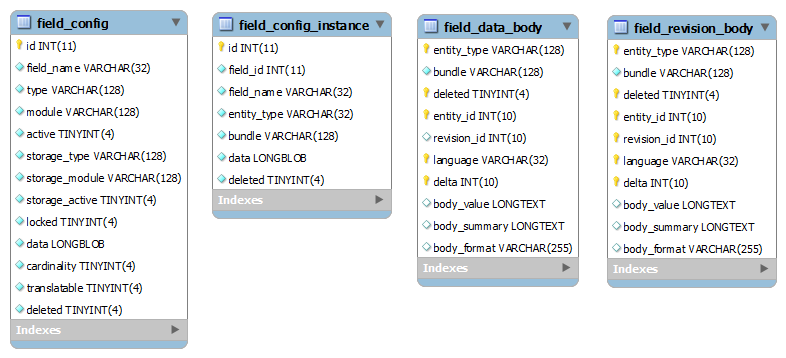
\includegraphics[width=1\textwidth]{fig/fieldtabellen}
\caption{Field tabellen}
\label{fig:fieldtabellen}
\end{figure}

\subsubsection{Aanmaken van Fields}
Velden kunnen aangemaakt worden met een GUI aangeboden door het Drupal systeem of ze kunnen aangemaakt worden vanuit code. Dit gebeurt dan best op het moment dat een module die ze nodig heeft ge\"{i}nstalleerd wordt, m.a.w. in de implementatie van hook\_install(). De velden worden aangemaakt met field\_create\_field(\$field) en de instanties worden aangemaakt met field\_create\_instance(\$instance). Hoe de argumenten voor deze functies opgebouwd zijn is beschikbaar in de Field CRUD API \cite{fieldCRUD}.

\subsubsection{Verwijderen van Fields}
Opnieuw kunnen velden verwijderd worden met een GUI aangeboden door het Drupal systeem of het kan vanuit code gebeuren. Via de GUI gebeurt dit impliciet door een contenttype te verwijderen. Achter de schermen wordt de functie node\_type\_delete(\$naam\_contenttype) opgeroepen en in deze functie wordt de functie field\_attach\_delete\_bundle(\$entity\_type, \$bundle) opgeroepen waar op zijn beurt de functie field\_delete\_instance(\$instance) oproept. Deze functies die achter de schermen opgeroepen worden wanneer de GUI gebruikt wordt, kunnen eveneens in code gebruikt worden.
\newpage
\subsection{Modules}
Een extra woordje uitleg hoe een module wordt toegevoegd en verwijderd uit een Drupal systeem kan geen kwaad. We merken meteen op dat er naast de\"{i}nstalleren van een module ook \textit{disablen} mogelijk is. Dit kan als gevolg hebben dat een beginnende Drupal ontwikkelaar veronderstellingen maakt die niet volledig kloppen. We maken een opsomming van handige feiten in verband met \textit{enablen}, \textit{disablen} en de\"{i}nstalleren voor beginnende Drupal ontwikkelaars:
\begin{itemize}
\item Bij \textit{disablen} wordt hook\_disable() opgeroepen. Dit is analoog voor \textit{enablen}, installeren en de\"{i}nstalleren.
\item Een gebruiker moet een module altijd eerst \textit{disablen} voor te de\"{i}nstalleren.
\item Een gebruiker kan een module enkel expliciet \textit{enablen}, \textit{disablen} of de\"{i}nstalleren. Een module wordt ge\"{i}nstalleerd als ze voor de eerste keer enabled wordt of eerst gede\"{i}nstalleerd werd voor te \textit{re-enablen}. Installeren kan dus enkel impliciet.
\item Sommige \textit{hooks} worden maar opgeroepen bij installatie van de module, wat betekent dat wanneer je een wijziging van deze \textit{hooks} wil doorvoeren, je de module moet \textit{disablen}, de\"{i}nstalleren en \textit{re-enablen}. De\"{i}nstallatie mag niet worden overgeslagen omdat de module dan niet geherinstalleerd wordt. Dit is van toepassing bij volgende \textit{hooks}:
\begin{itemize}
\item hook\_node\_info()
\item hook\_schema()
\end{itemize}
\end{itemize}

\subsection{Aanmaken en verwijderen van contenttypes}\label{contenttypeManipulatie}
\subsubsection{Aanmaken van contenttypes}
Er zijn meerdere manieren om contenttypes aan te maken en te configureren.
\begin{itemize}
\item Via een GUI die standaard aangeboden wordt door de Drupal website.
\item De functie node\_type\_save() gebruiken om een nieuw type op te slaan. Deze methode kan je overal in code gebruiken.
\item Hook\_node\_info() implementeren waarin je de nieuwe contenttypes beschrijft. Deze hook wordt enkel opgeroepen bij installatie van een module.
\end{itemize}
\noindent
De eerste optie is enkel interessant voor Drupal gebruikers die zelf geen module wensen aan te maken of voor ontwikkelaars die het effect op de databank van het aanmaken van een contenttype willen bekijken. De twee laatste functies kunnen door ontwikkelaars gebruikt worden om contenttypes aan te maken in code.De laatse optie wordt echter algemeen als de betere optie gezien omdat het gebruik van \textit{hooks} de \textit{Drupal way} is.
De laatste twee opties zijn echter niet voldoende om een contenttype volledig te configureren. Een aantal specifieke variabelen moeten toegevoegd worden in de \textit{variable}tabel. De variabelen die wij toevoegen, hebben een invloed op de configuratie van de contenttypes die we toevoegen.

De variabelen worden gezet in de implemenatie van hook\_enable() door de module die het contenttype definieert. Deze variabelen moeten voor elk contenttype gezet worden en bevatten de naam van het contenttype waar ze een invloed op hebben. Een volledige lijst van mogelijke variabelen die een invloed hebben op het contenttype vind je online \cite{contentTypeVariables}. We sommen degene op die we gebruiken:
\begin{itemize}
\item comment\_\textit{naam\_contenttype}: Krijgt de waarde 0 om \textit{default} commentaren uit te schakelen.
\item node\_options\_\textit{naam\_contenttype}: Krijgt de waarde array('status') om \textit{default} '\textit{Promote to Front page}' uit te vinken.
\item node\_preview\_\textit{naam\_contenttype}: Krijgt de waarde 0 om de mogelijkheid tot een preview te \textit{disablen}.
\item node\_submitted\_\textit{naam\_contenttype}: Krijgt de waarde 1 om \textit{default} de auteur en de tijd waarop de content is toegevoegd te tonen bij de content zelf.
\end{itemize}

\noindent
Een laatste stap die nog doorgevoerd moet worden is het cre\"{e}ren van de velden die toegevoegd gaan worden aan de contenttypes, vervolgens worden er instanties van de velden aangemaakt om ze te linken aan de contenttypes. Dit gebeurt in hook\_install(). Er worden velden aangemaakt voor: de URI van devices, de URI van resource en een veld voor meerdere referenties naar content van het type coap\_resource. Velden werden besproken in paragraaf~\ref{Fields}.

\subsubsection{Verwijderen van contenttypes}
De contenttypes worden verwijderd in hook\_uninstall(). Voor een contenttype kan verwijderd worden moeten nog een aantal andere zaken verwijderd worden. We overlopen de verschillende stappen die voor elk te verwijderen contenttype moeten overlopen worden:
\begin{itemize}
\item Alle content van het contenttype wordt verwijderd door middel van de functie\\ node\_delete\_multiple(\$nids). De variabele \$nid bevat een array met alle nids van de content die verwijderd wordt.
\item Alle variabelen die toegevoegd werden in de \textit{variable}tabel worden verwijderd door gebruik te maken van variable\_del(\$naam);
\item De comment-entiteit die geassocieerd is met dit contenttype wordt gemarkeerd om te verwijderen. Hiervoor wordt de functie field\_delete\_instance() gebruikt.
\item Het contenttype wordt verwijderd met node\_type\_delete(\$naam\_contenttype). In deze functie worden de instanties van de velden geassocieerd met dit contenttype ook verwijderd door gebruik te maken van de functie field\_attach\_delete\_bundle(\$entity\_type, \$bundle). We merken op dat de commentaren apart verwijderd werden.
\item De databankcache van node types wordt geupdated met node\_types\_rebuild(). Dit is nodig omdat Drupal vaak in caches kijkt en verouderde informatie kan gebruiken.
\item Drupal zal bij het verwijderen van velden de kolomwaarde deleted op 1 zetten. Om de velden effectief uit de databank te verwijderen wordt de functie field\_purge\_batch() gebruikt.
\end{itemize}

\newpage
\section{Database Abstraction Layer}\label{databaseAbstractionLayer}
Manipulatie van gegevens in de databank gebeurt via de \textit{Database Abstraction Layer} \cite{databaseAbstractionLayer}. Dit zorgt ervoor dat de implementatie van een module onafhankelijk is van de gebruikte soort databank. Concreet biedt deze laag een aantal functies aan voor het manipuleren van de databank. Wanneer een nieuw soort databank in gebruik genomen wordt, worden deze functies ge\"{i}mplementeerd voor deze nieuwe soort. We geven enkele voorbeelden van de meest gebruikte functies:

\scriptsize
\lstset{language=PHP}
\begin{lstlisting}[label=db_select,caption=Voorbeeld gebruik van db\_select]
$result = db_select('coap_sensor_interested_user','resource')
	->fields('resource', array('nid'))
	->condition('uri', $uri, '=')
	->condition('uid', $user->uid, '=')
	->execute();
\end{lstlisting}
\normalsize
In voorbeeld \ref{db_select} wordt opgevraagd wat het nid is voor een specifieke uri en uid. Er wordt gebruik gemaakt van de Drupalvariabele \$user. Zoals je ziet moet er een naam opgegeven worden na de tabelnaam. Deze naam moet herhaalt worden als eerste element van de fieldstabel. Merk op dat dit alleen nodig is bij het gebruik van db\_select. Als tweede element van de fieldstabel geef je een tabel op met alle velden die je wil opvragen. Meerdere condities kunnen opgegeven worden, de volgorde is niet belangrijk. De opgevraagde gegevens kunnen gesorteerd worden door gebruik te maken van -\textgreater orderBy('nid', 'ASC').\\

De variabele \$result zal een \textit{SelectQuery}-object bevatten. Er zijn twee manieren om de opgehaalde gegevens uit objecten van deze klasse te halen. Wanneer je weet dat er maar een enkele rij opgehaald wordt, doe je best het volgende

\scriptsize
\lstset{language=PHP}
\begin{lstlisting}
$record  = $result->fetchAssoc();
$nid = $record['nid'];
\end{lstlisting} 
\normalsize
Wanneer er meerdere rijen teruggegeven kunnen worden gebruik je beter

\scriptsize
\lstset{language=PHP}
\begin{lstlisting}
$nids = array();
foreach($result as $record){
	$nids[] = $record->nid;
}
\end{lstlisting}
\normalsize
om een tabel met al je gewenste resultaten in te bekomen. % In dit voorbeeld zal er echter maar \'{e}\'{e}n rij teruggegeven worden en is de eerste optie beter.

\newpage
\scriptsize
\lstset{language=PHP}
\begin{lstlisting}[label=db_insert,caption=Voorbeeld gebruik van db\_insert]
$id = db_insert('coap_sensor_interested_user')
	->fields(array(
		'uid' => $user->uid,
		'uri' => $resource_uri,
		'device' => 0,
		'nid' => $nid,
		'observe' => 0,
	))
	->execute();
\end{lstlisting}
\normalsize
In voorbeeld \ref{db_insert} wordt een entry toegevoegd aan de tabel coap\_sensor\_interested\_user. Kolommen die niet null mogen zijn en geen \textit{default}waarde hebben moeten opgegeven worden in de fieldstabel. Zoniet wordt er een exceptie opgegooid bij het oproepen van de execute-functie.

\scriptsize
\lstset{language=PHP}
\begin{lstlisting}[label=db_update,caption=Voorbeeld gebruik van db\_update]
$num_updated = db_update('coap_sensor_interested_user')
	->fields(array(
		'new' => 0,
	))
	->condition('uid', $user->uid, '=')
	->condition('device',1,'=')
	->condition('nid', $nid, '=')
	->execute();
\end{lstlisting}
\normalsize
In voorbeeld \ref{db_update} wordt van alle rijen die overeenstemmen met de opgegeven condities de new-waarde op 0 gezet. % Bij dit voorbeeld zal er maar \'{e}\'{e}n rij geupdated worden.

\scriptsize
\lstset{language=PHP}
\begin{lstlisting}[label=db_delete,caption=Voorbeeld gebruik van db\_delete]
db_delete('coap_sensor_interested_user')
	->condition('nid', $nid, '=')
	->execute();
\end{lstlisting}
\normalsize
In voorbeeld \ref{db_delete} worden alle rijen met als nid de waarde in \$nid verwijderd. % Opnieuw zal in dit voorbeeld maar \'{e}\'{e}n rij verwijderd worden.

\newpage
\section{JQuery in Drupal} \label{jQuery}
\begin{wrapfigure}{r}{0.25\textwidth}
\vspace{-40pt}
\hspace{-10pt}
\centering
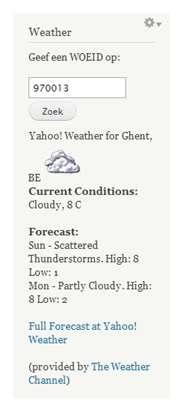
\includegraphics[width=0.3\textwidth]{fig/weermodule}
\vspace{-30pt}
\hspace{-10pt}
\centering
\caption{Weermodule}
\label{fig:weermodule}
%\centering
\vspace{-70pt}
\end{wrapfigure}

In deze paragraaf bekijken we hoe een module (weather\_info) gemaakt werd die het weerbericht ophaalt voor een regio naar keuze, aangegeven door een WOEID. In eerste instantie werd gewerkt met een formulier, maar in een latere fase werd overgestapt op jQuery, wat de gebruikerservaring bevordert.

\subsection{Met een HyperText Markup Language (HTML)-formulier} \nomenclature{HTML}{HyperText Markup Language}
In eerste instantie bevatte de module een formulier bestaande uit een tekstveld als invoer voor de WOEID en een knop om het formulier in te dienen.
Wanneer de gebruiker op de knop klikt, gebeuren volgende stappen:

\begin{itemize}
	\item het formulier wordt ingediend
	\item de pagina wordt opnieuw geladen
	\item de \textit{bootstrap}code roept hook\_form\_submit() op door weather\_location\_form\_submit() op te roepen (weather\_location is de naam van het formulier):
	\begin{itemize}
		\item het ingegeven WOEID wordt opgeslagen op serverniveau met de Drupal functie variable\_set()
	\end{itemize}
	\item de \textit{bootstrap}code roept hook\_block\_view op van de weermodule door weather\_info\_block\_view() op te roepen:
	\begin{itemize}
		\item het ingegeven WOEID wordt opgehaald met behulp van de Drupal functie variable\_get()
		\item er wordt een HTTP-\textit{request} uitgevoerd naar de \textit{Yahoo Weather API} met de PHP-functie file\_get\_contents(), dat een URL als parameter verwacht
		\item het ontvangen xml-bestand wordt in een object gestopt met de PHP-functie SimplexmlElement(), waarna het weerbericht gemakkelijk uit het XML-bestand kan gehaald worden
		\item Het weerbericht wordt toegevoegd aan de inhoud van het \textit{Block}
	\end{itemize}
	\item De pagina wordt in de browser weergegeven met het weerbericht in het \textit{Block}
\end{itemize}

\subsection{Met AJAX in jQuery}
Een pagina zal pas getoond worden wanneer de \textit{bootstrap} afgelopen is en aangezien de code in de \textit{hooks} die worden uitgevoerd onderdeel is van de \textit{bootstrap}, zal de pagina pas getoond worden wanneer de \textit{hooks} afgelopen zijn. Dit heeft als gevolg dat de gebruiker van de website langer moet wachten op de pagina omdat eerst nog een HTTP-\textit{request} moet gebeuren om het weerbericht op te halen. Het spreekt voor zich dat dit een zeer nadelig effect is dat moet vermeden worden.\\
Als alternatief hebben we gekozen om een jQuery-event te koppelen aan de submit-knop die het formulier indient. jQuery is namelijk geschreven in JavaScript en JavaScript is een \textit{client-side \textit{scripting} language}, wat inhoudt dat deze code wordt uitgevoerd op de machine van de gebruiker en dit nadat de pagina geladen is.\\
Wanneer de gebruiker op de knop klikt, wordt een \textit{Asynchronous JavaScript and XML}(AJAX)-\textit{call}\nomenclature{AJAX}{Asynchronous JavaScript and XML} uitgevoerd.
Zoals de naam suggereert, is dit een asynchrone aanroep, wanneer het antwoord aankomt, wordt automatisch een opgegeven functie opgeroepen waarin de data kan verwerkt worden. Als gevolg heeft de gebruiker dus geen enkele hinder van het internetverkeer dat noodzakelijk is om het weerbericht op te halen.

\subsection{Problemen}
JQuery laat geen \textit{cross-domain} AJAX \textit{calls} toe wegens veiligheidsoverwegingen. De \textit{Weather Service API} bevindt zich namelijk op een ander domein. Een oplossing hiervoor is een \textit{proxy}script in PHP gebruiken.
De AJAX-\textit{call} gebeurt dan naar het \textit{proxy}script dat zich op de server en dus hetzelfde domein bevindt. Het \textit{proxy}script vraagt daar effectief de data op en geeft de uitvoer terug.
De browser wordt dus eigenlijk om de tuin geleid. \cite{crossDomainProblem}
